\section{Lógica do controle aplicado}
\label{sec:logica_controle_aplicado}

Nesta seção explica-se a organização do sistema de controle da missão de \gls{rvdb}, isto é, a forma como as leis de controle, os modelos dinâmicos e os subsistemas auxiliares são habilitados, desabilitados e interconectados ao longo do tempo.
Serão detalhados:
(i) quais variáveis são consideradas entradas e saídas em cada etapa;
(ii) como as grandezas são convertidas entre referenciais para alimentar os sistemas subsequentes;
e (iii) quais critérios determinam as transições entre modos e a comutação para ativar o modo operacional do manipulador robótico.

A Figura~\ref{fig:geral_rvdb} apresenta o diagrama lógico geral da missão de \gls{rvdb}.
% ------------------------------------------------------------
\begin{figure}[H]
    \centering
    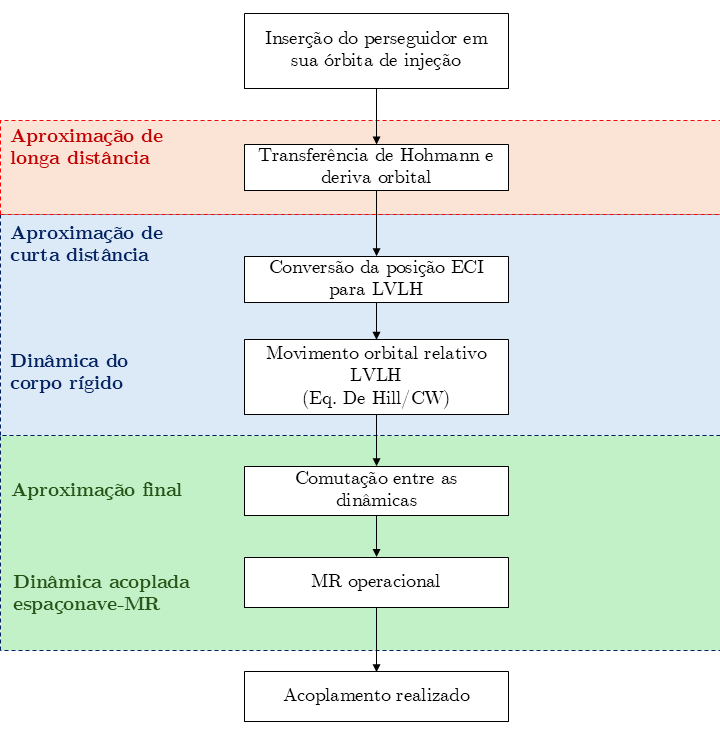
\includegraphics[width=0.7\linewidth]{3 Formulacao matematica/Imagens diagrama/1 Geral.png}
    \caption{Fluxo lógico geral da missão de \gls{rvdb}.}
    \label{fig:geral_rvdb}
\end{figure}
% ------------------------------------------------------------

A lógica é implementada como uma sequência de modos, que dependem do cumprimento de certas condições.
Em cada modo, utiliza-se simultaneamente: o modelo dinâmico ativo, as malhas de controle habilitadas e os limitadores de operação associados.
Essa estrutura separa as responsabilidades de cada subsistema ao longo da aproximação.
A etapa da aproximação de longa distância define a geometria relativa macroscópica por condição de fase e manobra impulsiva.
Por sua vez, a etapa da aproximação de curta distância conduz a aproximação controlada no referencial \gls{lvlh} com as respectivas restrições operacionais.
Por fim, a etapa de aproximação final efetua a transição para a dinâmica acoplada espaçonave--\gls{mr}, no qual a movimentação do manipulador robótico e seus efeitos de reação da espaçonave passam a influenciar a atitude da espaçonave.

A supervisão das transições incorpora condicionamento temporal para reduzir comutações instantâneas.
Como exemplo, a mudança do modo de operação do \gls{mr} não depende apenas de um limiar de posição relativa entre as espaçonaves no referencial \gls{lvlh}, mas da permanência dentro de uma janela geométrica por um intervalo de tempo mínimo. 
Dessa forma, busca-se evitar a alternância entre os modelos dinâmicos durante a passagem transitória pela região de acoplamento.
A partir disso, as subseções seguintes descrevem detalhadamente cada modo, os sinais que o alimentam e os sinais que ele produz, de forma direta com os diagramas de fluxo apresentados.

\subsection{Definição de eixos e convenção LVLH utilizada}
\label{subsec:definicao_eixos_convecao_lvlh}

O referencial \gls{lvlh} é definido com origem no centro de massa do alvo.
Neste trabalho adotou-se o formato utilizado por \cite{fehse2003}, portanto, o eixo along-track é alinhado com o vetor velocidade orbital do alvo, o eixo cross-track completa a mão direita.
Por sua vez, a componente radial é definida como a direção que aponta para o centro da Terra.
% Na implementação adotada, a componente radial do estado relativo em \gls{lvlh} é representada pela coordenada $z$ na direção do centro da Terra corresponde ao canal $-z$ no vetor de estado relativo utilizado nas leis de controle e na lógica de comutação.

%%%%%%%%%%%%%%%%%%%%%%% APP LONGA DISTANCIA

\subsection{Aproximação de longa distância}
\label{subsec:aprox_longa_distancia}

Inicialmente, o perseguidor é inserido pelo veículo lançador em sua órbita de injeção, enquanto que os elementos orbitais do alvo são assumidos conhecidos por informações da estação de solo, por exemplo.
Os elementos orbitais iniciais de ambas as espaçonaves são convertidos para o referencial ECI.
A evolução do movimento orbital das espaçonaves é obtida por propagação do problema de dois corpos para perseguidor e alvo, permitindo calcular o ângulo de fase entre as espaçonaves no referencial inercial.

A condição do início da transferência orbital é definida pelo ângulo de fase em ECI.
Uma vez satisfeita essa condição, aplica-se a transferência de Hohmann do tipo impulsiva, implementada por incrementos instantâneos de velocidade ($\Delta v$) no perseguidor.
Após a manobra, realiza-se um intervalo de deriva orbital para monitoramento, sem correções adicionais, com duração fixa de $5$ min, com o objetivo de verificar a posição e velocidade relativas antes de iniciar a formulação relativa em \gls{lvlh}.
A Figura~\ref{fig:app_longa} apresenta o diagrama lógico da aproximação de longa distância.
% ------------------------------------------------------------
\begin{figure}[H]
    \centering
    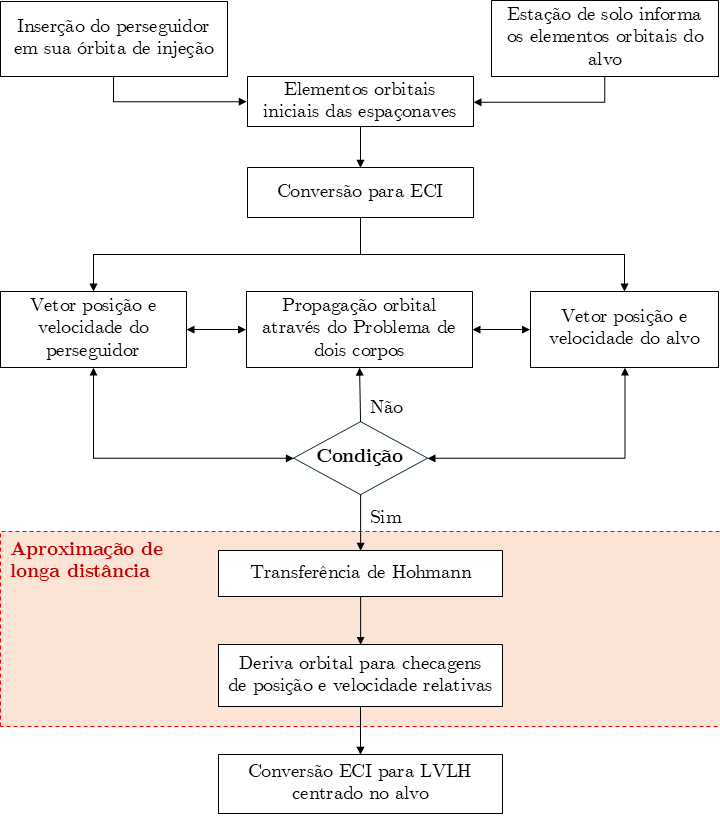
\includegraphics[width=\linewidth]{3 Formulacao matematica/Imagens diagrama/1 App longa.png}
    \caption{Fluxo lógico da aproximação de longa distância.}
    \label{fig:app_longa}
\end{figure}
% ------------------------------------------------------------
Ao final dessa etapa, os estados de perseguidor e alvo são convertidos de ECI para \gls{lvlh} centrado no alvo, obtendo-se o estado relativo (posição e velocidade relativas) e suas componentes em \gls{lvlh}, que passam a alimentar a etapa de aproximação de curta distância.

%%%%%%%%%%%%%%%%%%% APP CURTA DISTANCIA
\subsection{Aproximação de curta distância: dinâmica e lei de controle PD}
\label{subsec:aprox_curta_distancia_hcw_pd}

A etapa de aproximação de curta distância utiliza as equações lineares de \gls{hcw} (Equações~\ref{eq:equacoes_HillX}, \ref{eq:equacoes_HillY} e \ref{eq:equacoes_HillZ}) no referencial \gls{lvlh}, ainda assumindo órbita circular com referência no alvo.
Nesta fase, a dinâmica relativa fornece a evolução de posição e velocidade do perseguidor, e os comandos de controle são aplicados diretamente como acelerações de controle.
A Figura~\ref{fig:app_curta} apresenta o diagrama lógico da aproximação de curta distância.

% ------------------------------------------------------------
\begin{figure}[H]
    \centering
    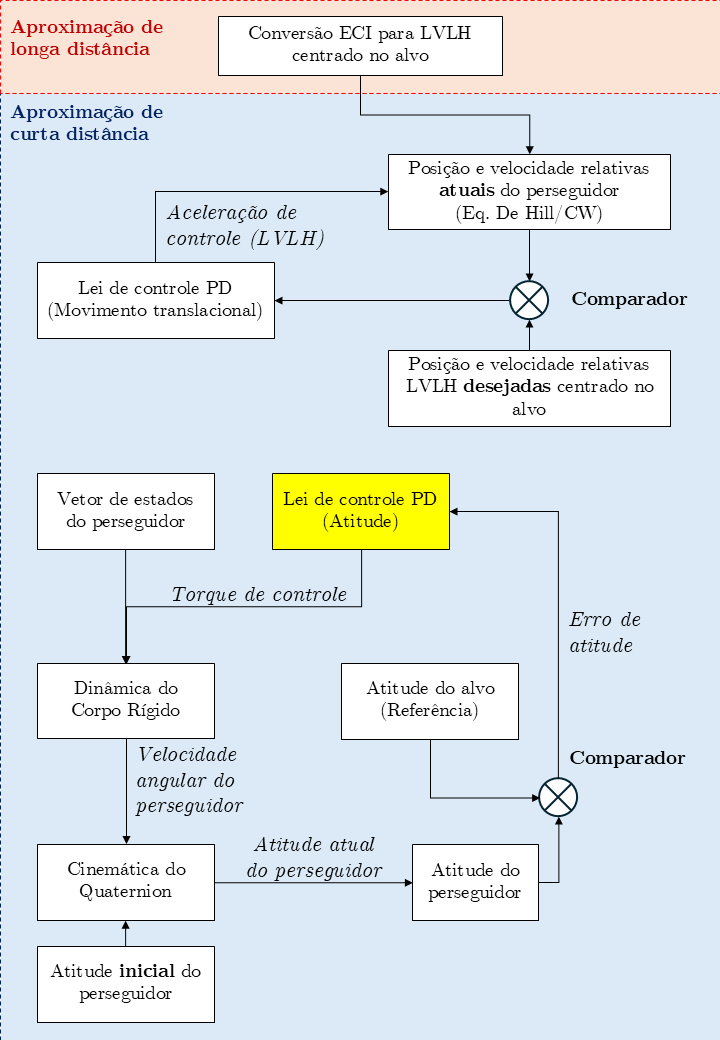
\includegraphics[width=0.7\linewidth]{3 Formulacao matematica/Imagens diagrama/2 App curta.png}
    \caption{Fluxo lógico da aproximação de curta distância em \gls{lvlh}.}
    \label{fig:app_curta}
\end{figure}
% ------------------------------------------------------------

\subsubsection{Lei de controle PD translacional}
\label{subsubsec:lei_pd_translacional_por_eixo}

A lei de controle translacional é implementada de forma individual, são três leis de controle PD independentes, uma por componente \gls{lvlh} (radial, along-track e cross-track).
Para cada eixo, a aceleração de comando é obtida a partir do erro de posição e do erro de velocidade em relação à referência, adotando velocidade desejada igual a zero.
Em seguida, aplica-se saturação na aceleração de comando por eixo, representando limites físicos ou de projeto.

Na implementação da lei de controle do eixo radial, a aceleração de comando é calculada como combinação linear proporcional--derivativa do erro de posição radial e do erro de velocidade radial, seguida por saturação em módulo. A mesma estrutura é aplicada aos demais eixos.

\subsubsection{Limitação de velocidade relativa na aproximação curta}
\label{subsubsec:limitacao_velocidade_relativa_curta}

Além da saturação em aceleração, conforme \cite{vedant2025longrange}, foi estabelecido limite na velocidade relativa, de modo a restringir a aproximação em curta distância a uma velocidade máxima de $0{,}03$ m/s quando o perseguidor está dentro de um limiar de distância de $20$ m. Fora desse limiar, admite-se limite de $0{,}30$ m/s.
A troca entre os limites é realizada por uma lógica do tempo mínimo dentro da faixa de distância relativa, isto é feito para evitar oscilações na transição das aproximações.
A velocidade limitada é então utilizada como entrada na lei de controle PD translacional.

\subsubsection{Lei de controle PD de atitude}
\label{subsubsec:lei_pd_atitude_quaternion}

Em paralelo ao controle translacional, durante a aproximação de curta distância, utiliza-se uma lei de controle PD para atitude baseada em quaternion.
A atitude desejada é a coincidência com o \gls{lvlh} centrado no alvo, o que corresponde a um quaternion desejado associado a essa orientação.
% Neste trabalho considerou $quat_{ref} = [1,0,0,0]$ como a atitude do alvo.

A atitude atual do perseguidor é propagada pela cinemática do quaternion, integrando a derivada do quaternion obtida a partir da velocidade angular.
A cada passo, o quaternion da atitude do perseguidor é normalizado para garantir unidade e proteção numérica.
Por fim, o erro de atitude é calculado por quaternion como o produto entre o quaternion desejado e o conjugado do quaternion atual, conforme \ref{eq:quat_relativo}.
% A parte vetorial do quaternion de erro é utilizada como sinal proporcional, enquanto a velocidade angular do corpo fornece o termo derivativo.
% O torque resultante é saturado por componentes, garantindo limites máximos de atuação.


%%%%%%%%%%%%%%%% APP FINAL

\subsection{Aproximação final e comutação de dinâmica}
\label{subsec:aprox_final_comutacao_dinamica}

A aproximação final é caracterizada pela ativação do modelo dinâmico acoplado entre espaçonave e o \gls{mr}.
Para que a comutação seja precisa e aconteça no momento certo, a mudança de modo depende de dois fatores:
(i) a posição relativa do perseguidor em \gls{lvlh} deve permanecer dentro de uma região de acoplamento definida por limites em along-track, cross-track e radial; 
e (ii) essa condição deve ser satisfeita continuamente por um tempo mínimo de condicionamento.
Enquanto o perseguidor não permanece na região pelo tempo necessário, mantém-se o modo anterior, ou seja dinâmica do corpo rígido calculado por \ref{eq:euler_corpo_rigido}.

Quando a comutação é realizada, são habilitados os seguintes subsistemas:

\begin{enumerate}[label=(\roman*)]
    \item a dinâmica acoplada via formulação de Lagrange, com desabilitação da dinâmica de corpo rígido via Euler em uma transição não instantânea;
    \item a cinemática inversa do \gls{mr};
    \item a cinemática direta e o cálculo dos Jacobianos linear e angular, incluindo a extração da posição do efetuador;
    \item a lei de controle PD das juntas do \gls{mr}.
\end{enumerate}
A Figura~\ref{fig:app_final} apresenta a relação dos subsistemas presentes no perseguidor.

% ------------------------------------------------------------
\begin{figure}[H]
    \centering
    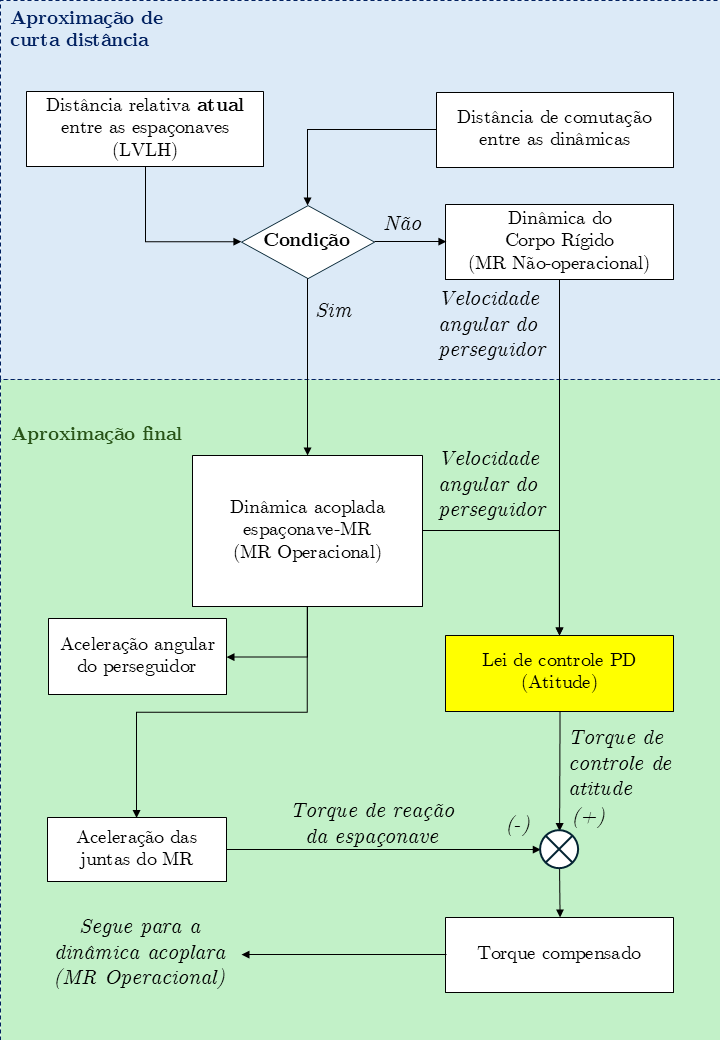
\includegraphics[width=0.7\linewidth]{3 Formulacao matematica/Imagens diagrama/3 App final.png}
    \caption{Comutação de dinâmica e ativação do modo operacional do \gls{mr}.}
    \label{fig:app_final}
\end{figure}
% ------------------------------------------------------------

%%%%%%%%%%%%%%%% TORQUE COMPENSADO

\subsubsection{Compensação do torque de reação do MR na atitude}
\label{subsubsec:compensacao_torque_reacao_atitude}

Durante o modo operacional do \gls{mr}, a movimentação dele induz torque de reação na espaçonave.
Esse efeito é compensado incluindo-se uma compensação em avanço no torque aplicado pela lei de controle PD de atitude, baseada em termos de acoplamento e Coriolis obtidos do modelo dinâmico total.
Na implementação, calcula-se o torque de reação como a contribuição do subsistema de acoplamento entre os graus de liberdade da espaçonave (3 de orientação) e do \gls{mr} multiplicada pela aceleração articular, somada ao termo de Coriolis correspondente à parte da espaçonave.
% O torque efetivamente aplicado na dinâmica acoplada é então dado por: torque compensado = torque da lei de controle PD de atitude $-$ torque de reação da espaçonave.
Essa estrutura busca manter o desempenho de seguimento de atitude durante movimentos do \gls{mr}, reduzindo perturbações induzidas pelo acoplamento dinâmico.

\subsection{Subsistema do MR: cinemática e controle articular}
\label{subsec:subsistema_mr_cinematica_controle}

O \gls{mr} é composto por três juntas revolutas.
No referencial 0 fixado à espaçonave, a junta 1 atua em torno do eixo $Z$ da espaçonave;
as juntas 2 e 3 atuam em torno do eixo $X$ da espaçonave.

A cadeia cinemática é utilizada para obter a pose do efetuador por cinemática direta e, a partir dela, calcular os Jacobianos linear e angular ($J_v$ e $J_w$) no referencial 0.

A partir da referência de aproximação do efetuador final (derivada da posição relativa do perseguidor em \gls{lvlh} e transformada para o referencial 0), a cinemática inversa gera comandos para o \gls{mr}, que são rastreados por uma lei de controle PD em espaço articular.
No modelo acoplado espaçonave--\gls{mr}, a dinâmica fornece diretamente as acelerações articulares; por integração, obtêm-se as velocidades e posições articulares utilizadas tanto no controle quanto na cinemática direta e nos Jacobianos.

A Figura~\ref{fig:mr_subsistema} apresenta a relação dos subsistemas presentes no perseguidor.
% ------------------------------------------------------------
\begin{figure}[H]
    \centering
    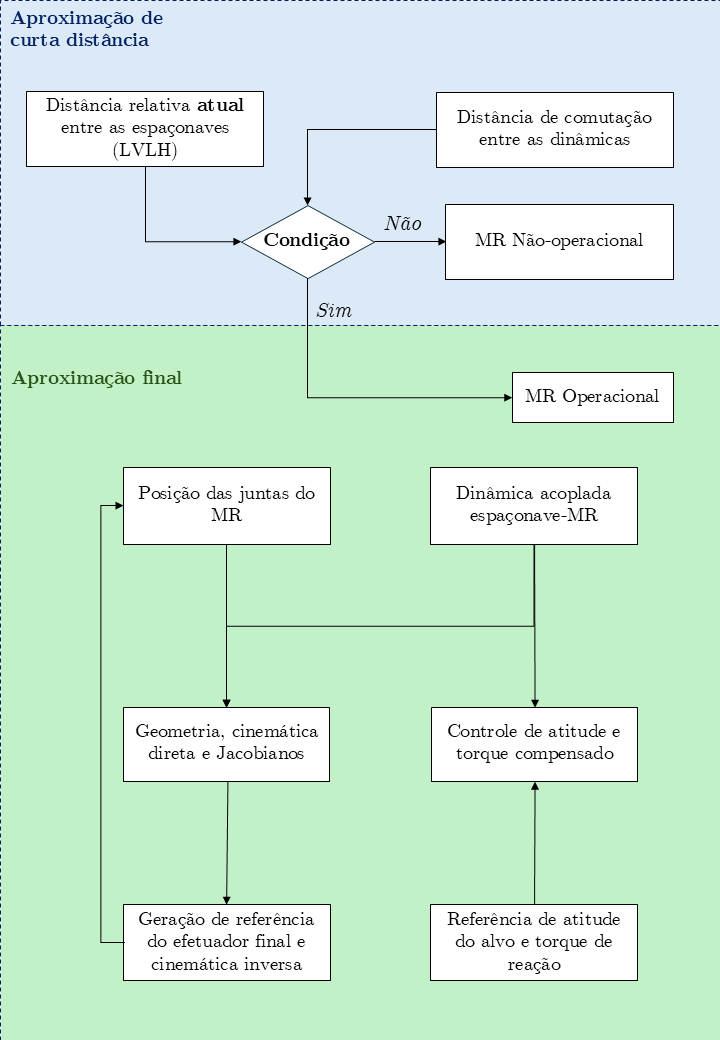
\includegraphics[width=0.7\linewidth]{3 Formulacao matematica/Imagens diagrama/4 MR.png}
    \caption{Blocos principais do subsistema do MR no modo operacional.}
    \label{fig:mr_subsistema}
\end{figure}
% ------------------------------------------------------------